\documentclass[12pt, a4paper]{article}
\usepackage[utf8]{inputenc}
\usepackage{amsmath}
\usepackage{relsize}
\usepackage{array}
\usepackage{xcolor}
\usepackage{courier}
\usepackage{listings}
\lstset{basicstyle=\footnotesize\ttfamily,breaklines=true}
\lstset{framextopmargin=50pt,frame=bottomline}
\usepackage{tikz}
\usetikzlibrary{calc}
\usepackage{graphicx}
\graphicspath{ {./images/} }

\title{CEG3155A Assignment 1}
\author{Jake Wang/*}
\date{\today}

\begin{document}
	\maketitle
	
	\section*{Question I}
	\subsection*{Part a}
	Use algebraic manipulation to show that for the three input variables $x_1$, $x_2$ and $x_3$
	\begin{equation}
		\sum{m(1,2,3,4,5,6,7) = x_1 + x_2 + x_3}
	\end{equation}

	Let $f = \sum{m(1,2,3,4,5,6,7)}$

	Then $f = (f')' = (\overline{x_1} \cdot \overline{x_2} \cdot \overline{x_3})' = x_1 + x_2 + x_3$ (De Morgan's Law)
	
	\subsection*{Part b}
	Use algebraic manipulation to show that for the three input variables $x_1$, $x_2$ and $x_3$
	\begin{equation}
		\prod{M(1,2,3,4,5,6,7) = x_1 \cdot x_2 \cdot x_3}
	\end{equation}

	Let $f = \prod{M(1,2,3,4,5,6,7)}$

	Then $f = (f')' = (\overline{x_1} + \overline{x_2} + \overline{x_3})' = x_1 \cdot x_2 \cdot x_3$
	
	
	\subsection*{Part c}
	Design the simplest circuit that realizes the function $f(x_1, x_2, x_3) = \sum{m(3, 4, 6, 7)}$ using \textbf{NAND gates only}.

	K-map:
	\begin{center}
		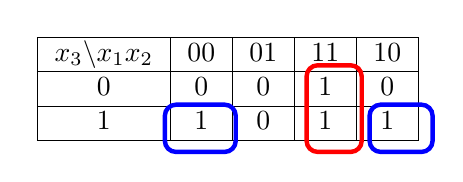
\begin{tikzpicture}
			\node(table)
			{
				\begin{tabular}{| c | c | c | c | c |}
					\hline
					$x_3$\textbackslash$x_1x_2$ & 00 & 01 & 11 & 10 \\
					\hline
					0 & 0 & 0 & 1 & 0 \\
					\hline
					1 & 1 & 0 & 1 & 1 \\
					\hline
				\end{tabular}
			};
			\draw [red, ultra thick, rounded corners] (1, -0.8) rectangle (1.7, 0.3);
			\draw [blue, ultra thick, rounded corners] (-0.8, -0.8) rectangle (0.1, -0.2);
			\draw [blue, ultra thick, rounded corners] (1.8, -0.8) rectangle (2.6, -0.2);
		\end{tikzpicture}
	\end{center}
	
	Convert to NAND representation:
	$$f(x_1, x_2, x_3) = \overline{\overline{x_1 x_2} \cdot \overline{\overline{x_2} x_3}}$$
	
	Design:\\
	\includegraphics[scale=0.5]{1c.png}
	
	\subsection*{Part d}
	Design the simplest circuit that realizes the function $f(x_1, x_2, x_3) = \sum{m(3, 4, 6, 7)}$ using \textbf{NOR gates only}.

	K-map:
	\begin{center}
		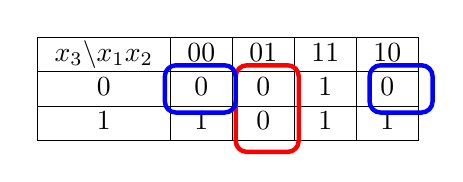
\begin{tikzpicture}
			\node(table)
			{
				\begin{tabular}{| c | c | c | c | c |}
					\hline
					$x_3$\textbackslash$x_1x_2$ & 00 & 01 & 11 & 10 \\
					\hline
					0 & 0 & 0 & 1 & 0 \\
					\hline
					1 & 1 & 0 & 1 & 1 \\
					\hline
				\end{tabular}
			};
			\draw [red, ultra thick, rounded corners] (0.1, -0.8) rectangle (0.9, 0.3);
			\draw [blue, ultra thick, rounded corners] (1.8, -0.3) rectangle (2.6, 0.3);
			\draw [blue, ultra thick, rounded corners] (-0.8, -0.3) rectangle (0.1, 0.3);
		\end{tikzpicture}
	\end{center}
	$$F(x_1, x_2, x_3) = (x_2 + x_3)(x_1 + \overline{x_2})$$
	
	Convert to NOR representation:
	$$F(x_1, x_2, x_3) = \overline{\overline{(x_2 + x_3)} + \overline{(x_1 + \overline{x_2})}}$$
	
	Design:\\
	\includegraphics[scale=0.5]{1d.png}
	
	
	\subsection*{Part e}
	Determine whether the following boolean functions are equal or not:
	\begin{equation}
		f(x, y, z) = x \cdot y + y \cdot z + \overline{x} \cdot z + \overline{x} \cdot \overline{y}
	\end{equation}
	\begin{equation}
		g(x, y, z) = x \cdot y + \overline{x} \cdot \overline{y} + \overline{x} \cdot y \cdot z
	\end{equation}

	\begin{align*}
		\begin{split}
			f(x, y, z)
			&= x \cdot y + y \cdot z + \overline{x} \cdot z + \overline{x} \cdot \overline{y} \\
			&= x \cdot y + \overline{x} \cdot \overline{y} + (y \cdot z + \overline{x} \cdot z) \\
			&= x \cdot y + \overline{x} \cdot \overline{y} + (\overline{x} + y) \cdot z
		\end{split}
	\end{align*}
	
	Since
	$$\overline{x} + y \not\equiv \overline{x} \cdot y$$
	
	Therefore, function $f$ and $g$ are not equivalent.
	
	\section*{Question II}
	\subsection*{Part a}
	Find the simplest realization for the function $f(x_1, ..., x_4) = {\sum{m(0, 3, 4, 7, 9, 10, 13, 14)}}$, assuming that the logic gates have a maximum fan-in of two.

	K-map:
	\begin{center}
		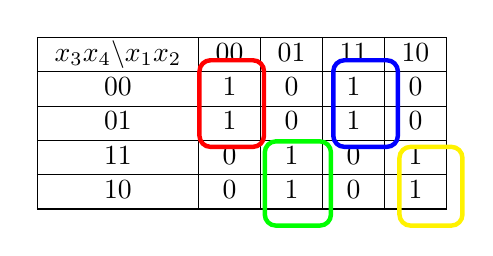
\begin{tikzpicture}
			\node(table)
			{
				\begin{tabular}{| c | c | c | c | c |}
					\hline
					$x_3x_4$\textbackslash$x_1x_2$ & 00 & 01 & 11 & 10 \\
					\hline
					00 & 1 & 0 & 1 & 0 \\
					\hline
					01 & 1 & 0 & 1 & 0 \\
					\hline
					11 & 0 & 1 & 0 & 1 \\
					\hline
					10 & 0 & 1 & 0 & 1 \\
					\hline
				\end{tabular}
			};
			\draw [red, ultra thick, rounded corners] (-0.54, -0.3) rectangle (0.28, 0.8);
			\draw [blue, ultra thick, rounded corners] (1.16, -0.3) rectangle (1.98, 0.8);
			\draw [green, ultra thick, rounded corners] (0.29, -1.3) rectangle (1.13, -0.23);
			\draw [yellow, ultra thick, rounded corners] (2, -1.3) rectangle (2.8, -0.3);
		\end{tikzpicture}
	\end{center}
	$$f = \overline{x_1} \cdot \overline{x_2} \cdot \overline{x_3} + \overline{x_1} \cdot x_2 \cdot x_3 + x_1 \cdot x_2 \cdot \overline{x_3} + x_1 \cdot \overline{x_2} \cdot x_3$$
	
	Simplification:
	\begin{align*}
	\begin{split}
	f
	&= \overline{x_1} \cdot (\overline{x_2} \cdot \overline{x_3} + x_2 \cdot x_3) + x_1 \cdot (x_2 \cdot \overline{x_3} + \overline{x_2} \cdot x_3) \\
	&= \overline{x_1} \cdot \overline{(x_2 \oplus x_3)} + x_1 \cdot (x_2 \oplus x_3) \\
	&= \overline{x_1 \oplus x_2 \oplus x_3}
	\end{split}
	\end{align*}
	
	Design with XOR/XNOR gates:\\
	\includegraphics[scale=0.41]{2aXOR.png}
	
	
	Design without XOR/XNOR gates:\\
	\includegraphics[scale=0.4]{2aNoXOR.png}
	
	
	\subsection*{Part b}
	Use the functional decomposition to find the best implementation for the function $f(x_1, ..., x_5) = \sum{m(1, 2, 7, 9, 10, 18, 19, 25, 31) + d(0, 15, 20, 26)}$. How does your realization compare with the cheapest SOP realization? Provide the costs.

	Let $d(0) = d(20) = 0$, $d(5) = d(26) = 1$

	Then:
	Let $g = x_5(x_1' + x_2)$, $f = g(x_3'x_4' + x_3x_4) + g'x_3'x_4$, assuming the maximum fan-in of each gate is 2:
	
	$$cost(g) = 2\ \text{gates} + 4\ \text{inputs} = 6$$
	$$cost(f) = 7\ \text{gates} + 14\ \text{inputs} = 21$$
	$$TotalCost = 6 + 21 = 27$$
	
	Cheapest SOP realization:
	$$h = x_3'x_4x_5' + x_1'x_3'x_4'x_5 + x_2x_3'x_4'x_5 + x_1x_2'x_3'x_4 + x_1'x_3x_4x_5 + x_2x_3x_4x_5$$

	$$cost(h) = 22\ \text{gates} + 44\ \text{inputs} = 66$$

	\subsection*{Part c}
	Use a Karnaugh map to minimize the next function boolean
	\begin{equation}
	\footnotesize{f(a, b, c, d, e) = {\sum{m(4, 5, 10, 11, 15, 18, 20, 24, 26, 30, 31) + d(9, 12, 14, 16, 19, 21, 25)}}}
	\end{equation}

	K-map:
	\begin{center}
		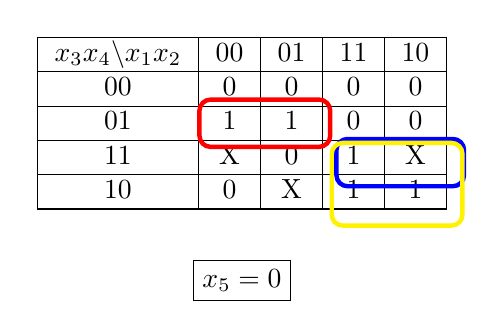
\begin{tikzpicture}
			\node(table)
			{
				\begin{tabular}{| c | c | c | c | c |}
					\hline
					$x_3x_4$\textbackslash$x_1x_2$ & 00 & 01 & 11 & 10 \\
					\hline
					00 & 0 & 0 & 0 & 0 \\
					\hline
					01 & 1 & 1 & 0 & 0 \\
					\hline
					11 & X & 0 & 1 & X \\
					\hline
					10 & 0 & X & 1 & 1 \\
					\hline
				\end{tabular}
			};
			\node[draw] at (0, -2) {$x_5 = 0$};
			\draw [red, ultra thick, rounded corners] (-0.54, -0.3) rectangle (1.12, 0.3);
			\draw [blue, ultra thick, rounded corners] (1.2, -0.8) rectangle (2.82, -0.2);
			\draw [yellow, ultra thick, rounded corners] (1.14, -1.3) rectangle (2.8, -0.25);
		\end{tikzpicture}
		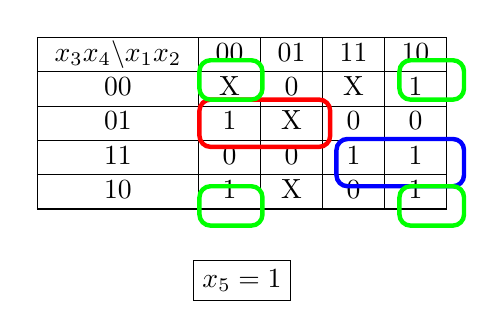
\begin{tikzpicture}
			\node(table)
			{
				\begin{tabular}{| c | c | c | c | c |}
					\hline
					$x_3x_4$\textbackslash$x_1x_2$ & 00 & 01 & 11 & 10 \\
					\hline
					00 & X & 0 & X & 1 \\
					\hline
					01 & 1 & X & 0 & 0 \\
					\hline
					11 & 0 & 0 & 1 & 1 \\
					\hline
					10 & 1 & X & 0 & 1 \\
					\hline
				\end{tabular}
			};
			\node[draw] at (0, -2) {$x_5 = 1$};
			\draw [red, ultra thick, rounded corners] (-0.54, -0.3) rectangle (1.12, 0.3);
			\draw [blue, ultra thick, rounded corners] (1.2, -0.8) rectangle (2.82, -0.2);
			\draw [green, ultra thick, rounded corners] (-0.54, -1.3) rectangle (0.26, -0.8);
			\draw [green, ultra thick, rounded corners] (-0.54, 0.3) rectangle (0.26, 0.8);
			\draw [green, ultra thick, rounded corners] (2, 0.3) rectangle (2.82, 0.8);
			\draw [green, ultra thick, rounded corners] (2, -1.3) rectangle (2.82, -0.8);
		\end{tikzpicture}
	\end{center}
	$$f = x_2'x_3x_4' + x_1'x_2x_4 + x_2x_3x_4 + x_1x_3'x_5'$$	

	\subsection*{Part d}
	Consider the following functions:
	\begin{equation}
	f_1 = \sum{m(0, 2, 4, 5, 9, 10, 11, 13, 15)}
	\end{equation}
	\begin{equation}
	f_2 = \sum{m(2, 5, 10, 11, 12, 13, 14, 15)}
	\end{equation}
	\begin{equation}
	f_3 = \sum{m(0, 2, 3, 4, 9, 11, 13, 14, 15)}
	\end{equation}
	
	Minimize these functions and realize them in a single least costly common circuit.
	
	$$f_1 = AD + A'B'D' + B'CD' + A'BC'$$
	$$f_2 = AC + AB + B'CD' + BC'D$$
	$$f_3 = AD + A'C'D' + A'B'C + ABC$$
	
	\section*{Question III}
	\subsection*{Part a}
	Consider the function $f = \overline{w_2} + \overline{w_1} \cdot \overline{w_3} + w_1 \cdot w_3$. Show how the repeated application of Shannon's expansion can be used to derive minterms of $f$.
	\begin{align*}
		\begin{split}	
			f
				&= w_1f(1, w_2, w_3) + w_1'f(0, w_2, w_3) \\
				&= w_1(w_2' + w_3) + w_1'(w_2' + w_3') \\
				&= w_1w_2' + w_1w_3 + w_1'w_2' + w_1'w_3' \\
				&= w_2f(w_1, 1, w_3) + w_2'f(w_1, 0, w_3) \\
				&= w_2(w_1w_3 + w_1'w_3') + w_2'(w_1 + w_1w_3 + w_1' + w_1'w_3') \\
				&= w_1w_2w_3 + w_1'w_2w_3' + w_1w_2' + w_1w_2'w_3 + w_1'w_2' + w_1'w_2'w_3' \\
				&= w_3f(w_1, w_2, 1) + w_3'f(w_1, w_2, 0) \\
				&= w_3(w_1w_2 + w_1w_2' + w_1'w_2') + w_3'(w_1'w_2 + w_1w_2' + w_1'w_2') \\
				&= f(1, 1, 1) + f(1, 0, 1) + f(0, 0, 1) + f(0, 1, 0) + f(1, 0, 0) + f(0, 0, 0) \\
				&= \sum{m(0, 1, 2, 4, 5, 7)}
		\end{split}
	\end{align*}

	\subsection*{Part b}
	Repeat part a for $f = w_2 + \overline{w_1} \cdot \overline{w_3}$.
	\begin{align*}
		\begin{split}	
			f
				&= w_2f(w_1, 1, w_3) + w_2'f(w_1, 0, w_3) \\
				&= w_2 + w_2'w_1'w_3' \\
				&= w_1f(1, w_2, w_3) + w_1'f(0, w_2, w_3) \\
				&= w_1w_2 + w_1'(w_2 + w_2'w_3') \\
				&= w_1w_2 + w_1'w_2 + w_1'w_2'w_3' \\
				&= w_3f(w_1, w_2, 1) + w_3'f(w_1, w_2, 0) \\
				&= w_3(w_1w_2 + w_1'w_2) + w_3'(w_1w_2 + w_1'w_2 + w_1'w_2') \\
				&= f(1, 1, 1) + f(0, 1, 1) + f(1, 1, 0) + f(0, 1, 0) + f(0, 0, 0) \\
				&= \sum{m(0, 2, 3, 6, 7)}
		\end{split}
	\end{align*}
	
	\subsection*{Part c}
	Derive the circuit of an 8-to-3 priority encoder.

	Assume the encoder has input $I_{7..0}$, output $O_{2..0}$, valid bit $V$.

	Truth table for the encoder:
	\begin{center}
		\begin{tabular}{| c | c | c | c | c | c | c | c || c | c | c || c |}
			\hline
			$I_7$ & $I_6$ & $I_5$ & $I_4$ & $I_3$ & $I_2$ & $I_1$ & $I_0$ & $O_2$ & $O_1$ & $O_0$ & $V$ \\
			\hline
			0 & 0 & 0 & 0 & 0 & 0 & 0 & 0 & 0 & 0 & 0 & 0 \\
			\hline
			0 & 0 & 0 & 0 & 0 & 0 & 0 & 1 & 0 & 0 & 0 & 1 \\
			\hline
			0 & 0 & 0 & 0 & 0 & 0 & 1 & X & 0 & 0 & 1 & 1 \\
			\hline
			0 & 0 & 0 & 0 & 0 & 1 & X & X & 0 & 1 & 0 & 1 \\
			\hline
			0 & 0 & 0 & 0 & 1 & X & X & X & 0 & 1 & 1 & 1 \\
			\hline
			0 & 0 & 0 & 1 & X & X & X & X & 1 & 0 & 0 & 1 \\
			\hline
			0 & 0 & 1 & X & X & X & X & X & 1 & 0 & 1 & 1 \\
			\hline
			0 & 1 & X & X & X & X & X & X & 1 & 1 & 0 & 1 \\
			\hline
			1 & X & X & X & X & X & X & X & 1 & 1 & 1 & 1 \\
			\hline
		\end{tabular}
	\end{center}
	$$O_2 = I_7 + I_7'I_6 + I_7'I_6'I_5 + I_7'I_6'I_5'I_4$$
	$$O_1 = I_7 + I_7'I_6 + I_7'I_6'I_5'I_4'I_3 + I_7'I_6'I_5'I_4'I_3'I_2$$
	$$O_0 = I_7 + I_7'I_6'I_5 + I_7'I_6'I_5'I_4'I_3 + I_7'I_6'I_5'I_4'I_3'I_2'I_1$$
	$$V = \sum_{i = 0}^{7}{I_i}$$

	Optimize output functions:
	$$O_2 = I_7 + I_6 + I_5 + I_4$$
	$$O_1 = I_7 + I_6 + I_5'I_4'I_3 + I_5'I_4'I_2 = I_7 + I_6 + I_5'I_4'(I_3 + I_2)$$
	$$O_0 = I_7 + I_6'I_5 + I_6'I_4'I_3 + I_6'I_4'I_2'I_1 = I_7 + I_6'(I_5 + I_4'(I_3 + I_2'I_1))$$
	
	Hardware Design:\\
	\includegraphics[scale=0.5]{3c.png}

	\subsection*{Part d}
	Perform the following functions using a 3-to-8 decoder:
	\begin{equation}
	f_1(a, b, c) = a \cdot b + \overline{a} \cdot \overline{b} \cdot {c}
	\end{equation}
	\begin{equation}
	f_2(a, b, c) = \overline{a} \cdot {b} + a \cdot \overline{b}
	\end{equation}
	
	$$f_1 = \sum{m(1, 6, 7)}$$
	$$f_2 = \sum{m(2, 3, 4, 5)}$$

	Hardware Design:\\
	\includegraphics[scale=0.6]{3d.png}

	\subsection*{Part e}
	Make a 6-to-64 decoder using four 4-to-16 decoders and one 2-to-4 decoder. Use $A_5A_4A_3A_2A_1A_0$ as data and $D_0 - D_{63}$ as outputs. Remember the signal Enable for each decoder.
	\\
	\includegraphics[scale=0.41]{3e.png}

	\section*{Question IV}
	\subsection*{Part a}
	Create an entity in VHDL called if2to4 which represents a binary 2-to-4 decoder, using an if-then-else expression. Give the VHDL code at the behavioral level. Create a second entity in VHDL called h3to8 which represents the binary 3-to-8 decoder shown in Figure 6.17, using two examples of the if2to4 entity. Write the code in VHDL at the structural level.
	
	\begin{lstlisting}[language=vhdl]
library ieee;
use ieee.std_logic_1164.all;

entity if2to4 is
    port(
        EN: in std_logic;
        I: in std_logic_vector(1 downto 0);
        O: out std_logic_vector(3 downto 0)
    );
end;

architecture Behaviourial of if2to4 is
begin
    process(I)
    begin
        if EN = '1' then
            if I = "00" then
                O <= "0001";
            elsif I = "01" then
                O <= "0010";
            elsif I = "10" then
                O <= "0100";
            else
                O <= "1000";
            end if;
        else
            O <= "0000";
        end if;
    end process;
end;
	\end{lstlisting}
	\begin{lstlisting}[language=vhdl]
library ieee;
use ieee.std_logic_1164.all;

entity h3to8 is
    port(
        I: in std_logic_vector(2 downto 0);
        O: out std_logic_vector(7 downto 0)
    );
end;

architecture Structural of h3to8 is
    component if2to4 is
        port(
            EN: in std_logic;
            I: in std_logic_vector(1 downto 0);
            O: out std_logic_vector(3 downto 0)
        );
    end component;
begin
    decoder1: if2to4
    port map(
        EN => I(2),
        I => I(1 downto 0),
        O => O(7 downto 4)
    );
    decoder0: if2to4
    port map(
        EN => not I(2),
        I => I(1 downto 0),
        O => O(3 downto 0)
    );
end;
	\end{lstlisting}

	\subsection*{Part b}
	Create an entity in VHDL called h6to64 which represents a 6-to-64 binary decoder. Use the treelike structure in Figure 6.18, in which the 6-to-64 decoder is constructed using five examples of the h3to8 decoder created in the problem in part a. Give the VHDL code at the structural level.
	
	\begin{lstlisting}[language=vhdl]
-- I don't believe it is possible to build a 6-to-64 decoder using only five 3-to-8 decoders,
-- since the total output width of five 3-to-8 decoders is only 40, which is significant lesser than 64.

-- So in my solution, I used a 9 instances of 3-to-8 decoder to build a 6-to-64 decoder.

library ieee;
use ieee.std_logic_1164.all;

entity h6to64 is
    port(
        EN: in std_logic;
        I: in std_logic_vector(5 downto 0);
        O: out std_logic_vector(63 downto 0)
    );
end;

architecture Structural of h6to64 is
    signal signalEnableControl: std_logic_vector(7 downto 0);
    component h3to8 is
        port(
            EN: in std_logic;
            I: in std_logic_vector(2 downto 0);
            O: out std_logic_vector(7 downto 0)
        );
    end component;
begin
    decoderController: h3to8
    port map(
        EN => EN,
        I => I(5 downto 3),
        O => signalEnableControl
    );
    
    decoder7: h3to8
    port map(
        EN => signalEnableControl(7) and EN,
        I => I(2 downto 0),
        O => O(63 downto 56)
    );

    decoder6: h3to8
    port map(
        EN => signalEnableControl(6) and EN,
        I => I(2 downto 0),
        O => O(55 downto 48)
    );

    decoder5: h3to8
    port map(
        EN => signalEnableControl(5) and EN,
        I => I(2 downto 0),
        O => O(47 downto 40)
    );

    decoder4: h3to8
    port map(
        EN => signalEnableControl(4) and EN,
        I => I(2 downto 0),
        O => O(39 downto 32)
    );

    decoder3: h3to8
    port map(
        EN => signalEnableControl(3) and EN,
        I => I(2 downto 0),
        O => O(31 downto 24)
    );

    decoder2: h3to8
    port map(
        EN => signalEnableControl(2) and EN,
        I => I(2 downto 0),
        O => O(23 downto 16)
    );

    decoder1: h3to8
    port map(
        EN => signalEnableControl(1) and EN,
        I => I(2 downto 0),
        O => O(15 downto 8)
    );

    decoder0: h3to8
    port map(
        EN => signalEnableControl(0) and EN,
        I => I(2 downto 0),
        O => O(7 downto 0)
    );
end;
	\end{lstlisting}

	\subsection*{Part c}
	Design a shift circuit, similar to the one in Figure 6.56, which can shift a vector of four input bits, $W = w_3w_2w_1w_0$, a one bit position to the right when the $Right$ control sign is equal to 1, and a one bit position to the left when the $Left$ control signal is 1. When both are 0 ($Right = Left = 0$), the circuit effciency should be the same as the input vector. Suppose the condition $Right = Left = 1$ will never occur.
	\begin{lstlisting}[language=vhdl]
library ieee;
use ieee.std_logic_1164.all;

entity MUX2x4 is
    port(
        D: in std_logic_vector(1 downto 0);
        I: in std_logic_vector(3 downto 0);
        O: out std_logic
    );
end;

architecture Structural of MUX2x4 is
begin
    with D select
        O <=
            I(0) when "00",
            I(1) when "01",
            I(2) when "10",
            I(3) when "11";
end;
	\end{lstlisting}
	\begin{lstlisting}[language=vhdl]
library ieee;
use ieee.std_logic_1164.all;

entity shift4bit is
    port(
        W: in std_logic_vector(3 downto 0);
        Left, Right: in std_logic;
        O: out std_logic_vector(3 downto 0)
    );
end;

architecture Structural of shift4bit is
    component MUX2x4 is
        port(
            D: in std_logic_vector(1 downto 0);
            I: in std_logic_vector(3 downto 0);
            O: out std_logic
        );
    end component;
begin
    MUX3: MUX2x4
    port map(
        D(1) => Left,
        D(0) => Right,
        I(3) => '0',
        I(2) => W(2),
        I(1) => '0',
        I(0) => W(3),
        O => O(3)
    );

    MUX2: MUX2x4
    port map(
        D(1) => Left,
        D(0) => Right,
        I(3) => '0',
        I(2) => W(1),
        I(1) => W(3),
        I(0) => W(2),
        O => O(2)
    );

    MUX1: MUX2x4
    port map(
        D(1) => Left,
        D(0) => Right,
        I(3) => '0',
        I(2) => W(0),
        I(1) => W(2),
        I(0) => W(1),
        O => O(1)
    );

    MUX0: MUX2x4
    port map(
        D(1) => Left,
        D(0) => Right,
        I(3) => '0',
        I(2) => '0',
        I(1) => W(1),
        I(0) => W(0),
        O => O(0)
    );
end;
	\end{lstlisting}
	
	\section*{Question V}
	\subsection*{Part a}
	Give the pseudo-code of that counter.

	\begin{lstlisting}[language=c]
		COUNT <- 0000; OUTPUT <- 0000;
		if (START)
			COUNT <- COUNT + 1;
			OUTPUT <- COUNT XOR (COUNT >> 1);
		else
			COUNT <- 0000;
			OUTPUT <- 0000;
		Go back to the first if statement;
	\end{lstlisting}

	\subsection*{Part b}
	Using the pseudo-code above, your task is to design and demonstrate the ASM diagram (in graphic format), the datapath, the detailed ASM diagram (in graphical format) and the controlpath performed with the method of a state flip-flop. Note that you can take the output of the counter as the output of a set of 1-bit registers.
	
	ASM Diagram:\\
	\includegraphics[scale=0.8]{5bASM.pdf}

	Datapath:\\
	\begin{center}
		\includegraphics[scale=0.8]{5bDatapath.pdf}
	\end{center}
	
	Detailed ASM Diagram:\\
	\includegraphics[scale=0.8]{5bDetailedASM.pdf}

	Control Logic Diagram:\\
	\includegraphics{5bControlLogic.pdf}

	\section*{Bonus Question}
	Show that if two 2's complement numbers are added, the overflow bit is the XOR of the carry-in and carry-out of the most significant bit (MSB).
	\\

	Overflow only occurs when two positive numbers or two negative numbers add together.
	\\

	Case 1: When two positive numbers add together. According to the definition of 2's complement numbers, the MSB of two positive numbers should be 0. Hence, the carry-out of MSB should be 0 in any case.

	If the carry-in of MSB is 0, the result will still be a positive number, no overflow. However, if the carry-in of MSB is 1, the result will be a negative number---overflow occurred. 
	\\

	Case 2: When two negative numbers add together. Similarly, the MSB of two negative numbers should be 1 and the carry-out of MSB should be 1 in any case.

	If the carry-in of MSB is 1, the result will still be a negative number---no overflow. But if the carry-in of MSB is 0, the result will be a positive number---overflow occurred.
	\\

	From above two cases, it is shown that if the carry-in and carry-out of MSB are different, there is an overflow. Thus, an XOR gate can be applied to the carry-in and carry-out of MSB to detect overflow.

\end{document}
